% ==========================================================
% ENTREGA 1 — A pergunta do trabalho
% Teoria do Aprendizado Estatístico — Ciências de Dados
% Fatec Baixada Santista – Rubens Lara
% Derivado de modelo-trabalho.Rnw (R + knitr + abnTeX2)
% ==========================================================
%
% O QUE ENTREGAR
%   Um texto de NO MÁXIMO 3 PÁGINAS, com quatro seções:
%     1. Introdução ................... o contexto e o objetivo
%     2. O banco de dados e o problema  a escolha e a motivação dela
%     3. A pergunta ................... a pergunta e a ficha de 7 campos
%     4. Defesa da pergunta ........... a evidência de que ela se sustenta
%   Mais as Referências (não contam nas 3 páginas).
%
% ONDE ENTREGAR
%   O PDF e este .Rnw em  consolidados/
%   O código que gerou os números em  estrutura/codigo/
%
% COMO COMPILAR
%   RStudio: Tools > Global Options > Sweave >
%            "Weave Rnw files using: knitr" e "Typeset LaTeX into PDF using: pdfLaTeX".
%            Depois, botão "Compile PDF".
%   Terminal: Rscript -e "knitr::knit2pdf('entrega-1-pergunta.Rnw')"
%
% ARQUIVOS NECESSÁRIOS NA MESMA PASTA
%   entrega-1-pergunta.Rnw   (este arquivo)
%   referencias.bib          (as referências em BibTeX)
%
% REQUISITOS
%   R com knitr; LaTeX com abntex2 (TeX Live: texlive-publishers).
%   Salve em UTF-8. Se acentos saírem como <U+00E9>, a sessão do R não
%   está em locale UTF-8 (Linux: LANG=pt_BR.UTF-8 ou C.UTF-8).
% ==========================================================

\documentclass[
  article,
  12pt,
  oneside,
  a4paper,
  english,
  brazil
]{abntex2}\usepackage[]{graphicx}\usepackage[]{xcolor}
% maxwidth is the original width if it is less than linewidth
% otherwise use linewidth (to make sure the graphics do not exceed the margin)
\makeatletter
\def\maxwidth{ %
  \ifdim\Gin@nat@width>\linewidth
    \linewidth
  \else
    \Gin@nat@width
  \fi
}
\makeatother

\definecolor{fgcolor}{rgb}{0.345, 0.345, 0.345}
\newcommand{\hlnum}[1]{\textcolor[rgb]{0.686,0.059,0.569}{#1}}%
\newcommand{\hlsng}[1]{\textcolor[rgb]{0.192,0.494,0.8}{#1}}%
\newcommand{\hlcom}[1]{\textcolor[rgb]{0.678,0.584,0.686}{\textit{#1}}}%
\newcommand{\hlopt}[1]{\textcolor[rgb]{0,0,0}{#1}}%
\newcommand{\hldef}[1]{\textcolor[rgb]{0.345,0.345,0.345}{#1}}%
\newcommand{\hlkwa}[1]{\textcolor[rgb]{0.161,0.373,0.58}{\textbf{#1}}}%
\newcommand{\hlkwb}[1]{\textcolor[rgb]{0.69,0.353,0.396}{#1}}%
\newcommand{\hlkwc}[1]{\textcolor[rgb]{0.333,0.667,0.333}{#1}}%
\newcommand{\hlkwd}[1]{\textcolor[rgb]{0.737,0.353,0.396}{\textbf{#1}}}%
\let\hlipl\hlkwb

\usepackage{framed}
\makeatletter
\newenvironment{kframe}{%
 \def\at@end@of@kframe{}%
 \ifinner\ifhmode%
  \def\at@end@of@kframe{\end{minipage}}%
  \begin{minipage}{\columnwidth}%
 \fi\fi%
 \def\FrameCommand##1{\hskip\@totalleftmargin \hskip-\fboxsep
 \colorbox{shadecolor}{##1}\hskip-\fboxsep
     % There is no \\@totalrightmargin, so:
     \hskip-\linewidth \hskip-\@totalleftmargin \hskip\columnwidth}%
 \MakeFramed {\advance\hsize-\width
   \@totalleftmargin\z@ \linewidth\hsize
   \@setminipage}}%
 {\par\unskip\endMakeFramed%
 \at@end@of@kframe}
\makeatother

\definecolor{shadecolor}{rgb}{.97, .97, .97}
\definecolor{messagecolor}{rgb}{0, 0, 0}
\definecolor{warningcolor}{rgb}{1, 0, 1}
\definecolor{errorcolor}{rgb}{1, 0, 0}
\newenvironment{knitrout}{}{} % an empty environment to be redefined in TeX

\usepackage{amsmath}
\usepackage{alltt}

\usepackage[T1]{fontenc}
\usepackage[utf8]{inputenc}
\usepackage{lmodern}
\usepackage{amsmath,amssymb}
\usepackage{icomma}
\usepackage{booktabs}
\usepackage[alf]{abntex2cite}

\hypersetup{hidelinks}

% ----------------------------------------------------------
% DADOS DA ENTREGA — preencha aqui
% ----------------------------------------------------------
\titulo{A pergunta do trabalho: \textit{escreva aqui a sua pergunta, em uma linha}}
% O abntex2 imprime um "titulo estrangeiro" logo abaixo do titulo quando o
% documento declara mais de um idioma. Deixe vazio se nao houver.
\tituloestrangeiro{}
\autor{Nome do Grupo}
\local{Santos-SP}
\data{\today}

\newcommand{\nomecurso}{Tecnologia em Ciência de Dados}
\newcommand{\nomedisciplina}{Teoria do Aprendizado Estatístico}
\newcommand{\nomeprofessor}{Prof.\ Dr.\ João Paulo Ferreira de Mello}
\newcommand{\repositorio}{projeto-nome-do-grupo}
% Um integrante por linha: Nome Completo -- RA
\newcommand{\integrantes}{%
  Nome Completo do Integrante 1 -- RA 0000000000000 \\
  Nome Completo do Integrante 2 -- RA 0000000000000 \\
  Nome Completo do Integrante 3 -- RA 0000000000000%
}
\IfFileExists{upquote.sty}{\usepackage{upquote}}{}
\begin{document}





\selectlanguage{brazil}
\frenchspacing

% ----------------------------------------------------------
% IDENTIFICAÇÃO
% ----------------------------------------------------------
\maketitle

\begin{center}
  \small
  Fatec Baixada Santista -- Rubens Lara \\
  \nomecurso{} \quad|\quad \nomedisciplina{} \quad|\quad \nomeprofessor{} \\[0.4em]
  \integrantes \\[0.4em]
  Repositório: \texttt{\repositorio}
\end{center}

\textual

% ==========================================================================
\section{Introdução}
% ==========================================================================
% ~meia página. O QUE VAI AQUI:
%   - de que assunto trata o trabalho (o domínio, em linguagem comum);
%   - por que esse assunto importa, e para quem;
%   - o que este texto entrega: a pergunta que o grupo vai perseguir
%     no resto do semestre, e a evidência de que ela se sustenta.
% NÃO adiante aqui os números da Seção 4.

Apresente o domínio do trabalho e diga por que ele interessa. Feche o primeiro
parágrafo dizendo, em uma frase, o que este texto faz: apresenta o banco
escolhido, formula a pergunta do trabalho e mostra que os dados têm condição de
respondê-la.

Referências entram pela NBR 10520. Com o autor ao fim da frase, o formato sai
entre parênteses \cite{james2021}; com o autor no corpo do texto, use
\verb|\citeonline| --- segundo \citeonline{bruce2019}, a escolha da métrica vem
antes da escolha do modelo. Para indicar página: \cite[p.~23]{james2021}.

% ==========================================================================
\section{O banco de dados e o problema}
% ==========================================================================
% ~três quartos de página. O QUE VAI AQUI:
%   - ORIGEM: de onde veio o banco (órgão, portal, empresa, coleta própria),
%     com a referência bibliográfica e a data de acesso;
%   - CONTEÚDO: o que é uma LINHA (uma pessoa? um mês? uma transação?),
%     quantas linhas, quantas colunas, quais são as principais;
%   - MOTIVAÇÃO: por que este banco, e não outro. Responda honestamente:
%     foi interesse pelo assunto? disponibilidade? experiência prévia
%     do grupo? Todas são razões legítimas -- o que não vale é não ter
%     razão nenhuma;
%   - O PROBLEMA: que decisão, no mundo real, depende desse assunto.

Descreva a origem do banco, com a referência \cite{fonte_dados}. Diga o que
representa cada linha e quais são as colunas principais. O conjunto usado tem
$n = \text{150}$ observações e $p = \text{4}$ preditores candidatos.

Explique a escolha: por que este banco. E termine situando o \emph{problema} ---
a decisão concreta, tomada por alguém, que dependeria de uma resposta melhor do
que a que se tem hoje.

% ==========================================================================
\section{A pergunta}
% ==========================================================================
% ~três quartos de página. O QUE VAI AQUI:
%   - a pergunta em UMA FRASE, sem jargão -- alguém de fora da área
%     precisa entendê-la;
%   - a ficha de sete campos preenchida (Tabela 1);
%   - um parágrafo justificando o TIPO: por que regressão e não
%     classificação (ou o contrário), e por que predição e não inferência.

Enuncie aqui a pergunta, em uma frase, sem jargão técnico. A
Tabela~\ref{tab:ficha} detalha os sete campos que a definem.

\begin{table}[htb]
  \centering
  \caption{Ficha da pergunta}
  \label{tab:ficha}
  \small
  \begin{tabular}{@{}p{0.30\textwidth}p{0.62\textwidth}@{}}
    \toprule
    \textbf{Campo} & \textbf{Preenchimento} \\
    \midrule
    1. A pergunta, em uma frase & \textit{escreva aqui} \\
    2. Resposta $Y$: coluna, tipo, unidade & \texttt{Sepal.Length} ---
       quantitativa --- \textit{unidade} \\
    3. Preditores $X$: quais e quantos & \textit{liste} \quad ($p = \text{4}$) \\
    4. Tipo: as três decisões & supervisionado; regress\~ao;
       \textit{predição ou inferência?} \\
    5. Métrica & RMSE, na unidade de $Y$ \\
    6. Linha de base a bater & RMSE = 0,83 \quad (chutar sempre a m\'edia) \\
    7. Dono do problema & \textit{quem decidiria o quê com a resposta?} \\
    \bottomrule
  \end{tabular}
  \fonte{Elaborada pelos autores.}
\end{table}

Justifique o tipo escolhido. Lembre que o campo 7 é o que separa uma pergunta de
um exercício: se ninguém decidiria nada diferente com a resposta, a pergunta
precisa ser reformulada.

% ==========================================================================
\section{Defesa da pergunta}
% ==========================================================================
% ~uma página. É A SEÇÃO QUE PESA MAIS. O QUE VAI AQUI:
%   - o diagnóstico do banco (Tabela 2), comentado item a item;
%   - a passagem pelos quatro descartes: vazamento, n contra p, balanço
%     de classes, faltantes -- dizendo o que foi encontrado e o que o
%     grupo fez a respeito;
%   - a figura da resposta (Figura 1), com uma frase de leitura;
%   - o veredito: a pergunta se sustenta? Se um descarte pegou, o que
%     mudou na pergunta por causa dele?
% Os números desta seção saem do bloco <<dados>> -- eles se atualizam
% sozinhos quando voces trocarem o banco.

A Tabela~\ref{tab:diag} reúne as quatro verificações feitas sobre o banco.

\begin{table}[htb]
  \centering
  \caption{Diagnóstico do banco}
  \label{tab:diag}
  \small
  \begin{tabular}{@{}p{0.32\textwidth}p{0.60\textwidth}@{}}
    \toprule
    \textbf{Verificação} & \textbf{Resultado} \\
    \midrule
    Tamanho ($n \times p$)   & $\text{150} \times \text{4}$ \\
    Linha de base            & RMSE = 0,83 \quad (chutar sempre a m\'edia) \\
    Maior correlação com $Y$ & \texttt{Petal.Length}: 0,872 \\
    Balanço das classes      & n\~ao se aplica (resposta quantitativa) \\
    Valores faltantes        & nenhum \\
    \bottomrule
  \end{tabular}
  \fonte{Elaborada pelos autores.}
\end{table}

\textbf{Vazamento.} A linha ``maior correlação'' da Tabela~\ref{tab:diag}
aponta o preditor mais parecido com a resposta. Diga se essa semelhança é
natural ou se denuncia uma coluna que \emph{já contém} a resposta --- e, nesse
caso, o que foi removido. Quando a resposta é qualitativa a correlação não se
aplica: verifique coluna a coluna se alguma separa as classes quase
perfeitamente.

\textbf{Tamanho.} São $\text{150}$ observações para $\text{4}$ preditores.
Comente se há observações suficientes por coluna, e o que isso implica para a
escolha do modelo.

\textbf{Balanço e faltantes.} Comente o balanço das classes (quando a resposta
for qualitativa) e a presença de valores faltantes, dizendo o que o grupo
pretende fazer com eles.

A Figura~\ref{fig:resposta} mostra a distribuição da resposta.

\begin{figure}[htb]
  \centering
  \caption{Distribuição da resposta \texttt{Sepal.Length}}
  \label{fig:resposta}
\begin{knitrout}
\definecolor{shadecolor}{rgb}{0.969, 0.969, 0.969}\color{fgcolor}

{\centering 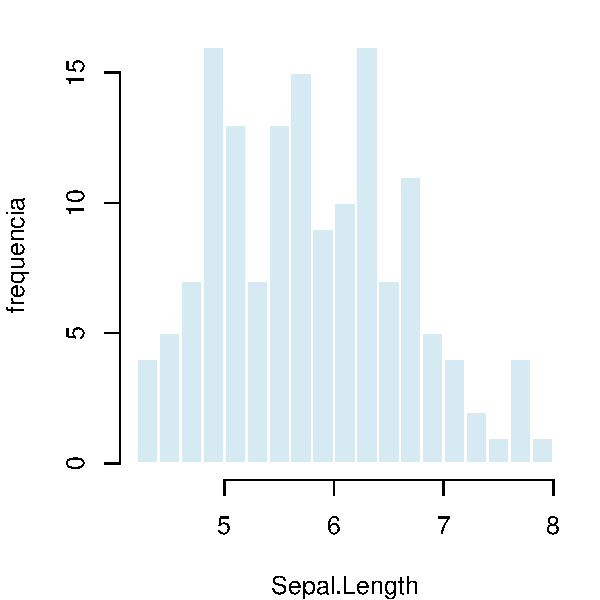
\includegraphics[width=0.52\linewidth]{figure/fig-resposta-1} 

}


\end{knitrout}
  \fonte{Elaborada pelos autores.}
\end{figure}

\textbf{Veredito.} Feche dizendo se a pergunta se sustenta. Se algum descarte
pegou, diga o que mudou na pergunta por causa dele --- uma pergunta corrigida
por evidência vale mais do que uma pergunta que nunca foi testada.

A pergunta é \textbf{provisória}: será revista depois da Aula 12, quando o
grupo tiver o kit supervisionado completo. Registre em uma frase o que as
próximas aulas podem mudar nesta resposta.

% ----------------------------------------------------------
% REFERÊNCIAS — não contam nas 3 páginas.
% Só aparecem as obras citadas. Para incluir uma obra não citada,
% use \nocite{chave}.
% ----------------------------------------------------------
\postextual
\bibliography{referencias}

\end{document}
